\documentclass[lettersize,journal]{IEEEtran}
\usepackage{amsmath,amsfonts}
\usepackage{algorithmic}
\usepackage{algorithm}
\usepackage{array}
\usepackage[caption=false,font=normalsize,labelfont=sf,textfont=sf]{subfig}
\usepackage{textcomp}
\usepackage{stfloats}
\usepackage{url}
\usepackage{verbatim}
\usepackage{graphicx}
\usepackage{cite}
\usepackage{longtable} % for tables
\usepackage{booktabs} % for tables

\hyphenation{op-tical net-works}
\setlength{\parindent}{0pt}

\begin{document}

\title{Neural Networks-Deep Learning \\ 2nd Assignment}
\author{Papadakis Konstantinos Fotios}
% The paper headers
\markboth{Neural Networks-Deep Learning, 2nd Assignment, 2024}
\maketitle

\textbf{Author:} Papadakis Konstantinos Fotios \\

\smallskip

\begin{abstract}
This is the second Assignment of the course "Neural Networks-Deep Learning". It revolves around
creating a Support Vector Machine and and training it on the CIFAR-10 dataset to successfully 
classify the images into one of the 10 classes. The algorithm used is analyzed extensively and
results both in the testing and training phase are presented. SVM is challenged by other similar
algorithms that are also trained on the CiFAR-10 dataset and try to solve the same classification 
problem. These rival algorithms include 1 and 3 Nearest Neighbor, Nearest Centroid and MLP with
one hidden layer using Hinge loss.
\end{abstract}

\section{Introduction}
\IEEEPARstart{T}{he} second assignment is going to utilize results from the first assignment and
thus the dataset has to be the same: "CIFAR-10".
\begin{itemize}
  \item \url{https://www.cs.toronto.edu/~kriz/cifar.html}
\end{itemize}

It consists of 60000 32x32 color images which belong to one of the 10 available classes. There are
6000 images per class, 5000 training images and 1000 test images. The data is available in 6 
batches of 10000 images each.
\begin{itemize}
  \item five training batches (50,000 or 5000 images from each class)
  \item one test batch (10,000 or 1000 images from each class)
\end{itemize}
Since the training batches' images are chosen randomly, each batch individually may contain more 
images from one class than another but, cumulatively, the number of images from each class is 
equal. Here is an example of the dataset's structure:

\begin{figure}[H]
  \centering
  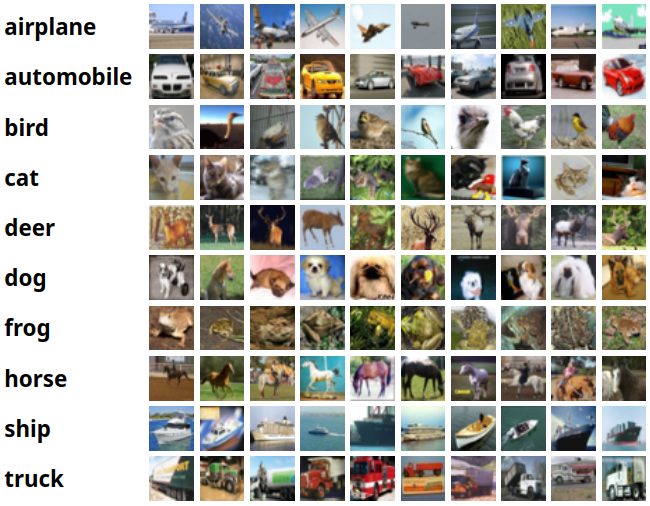
\includegraphics[width=2.5in]{media/cifar10_example.png}
  \caption{The CIFAR-10 dataset.}
  \label{CIFAR example}
\end{figure} 

\section{Support Vector Machine}
Support Vector Machines are supervised maximum margin models that are used for problems 
such as:
\begin{itemize}
    \item Classification
    \item Regression
    \item Distribution Estimation
\end{itemize}
They are considered supervised because they need a pre-labeled training set to develop 
the hyperplanes that separate the classes. The terminology maximum margin refers to the
fact that the SVM tries to solve a convex optimization problem which maximizes the 
distance between the hyperplane and the closest data points from each class. This 
distance is called "margin".

\begin{figure}[H]
    \centering
    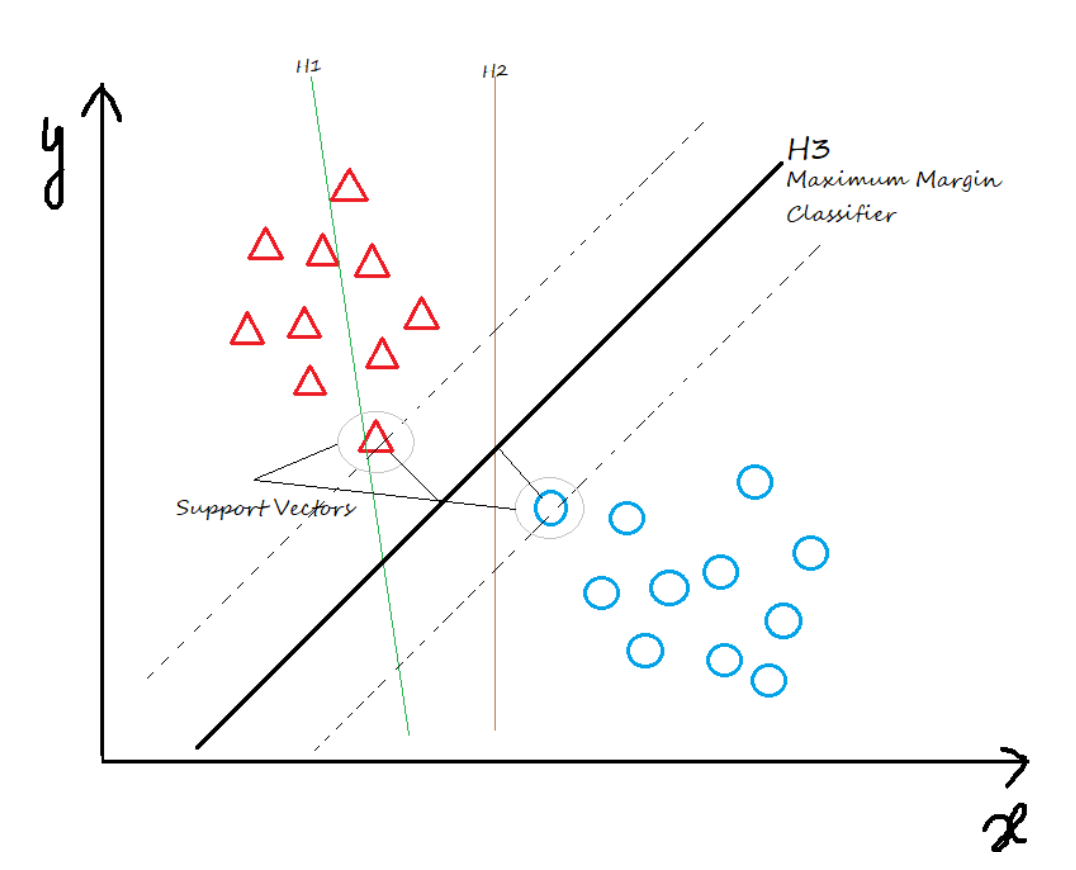
\includegraphics[width=0.5\textwidth]{media/svm_example.png}
    \caption{SVM Maximum Margin Classifier}
\end{figure}


\section{Nearest Neighbor and Nearest Centroid}
First nearest neighbor, third nearest neighbor and nearest centroid are three basic
classification algorithms we will be taking from the first assignment to compare our
SVM with. These as we have explained previously are algorithms that classify by:
\begin{itemize}
    \item Nearest Neighbor: Assigns to the test point the class of the nearest to it 
    centroid calculated from all the points in the training dataset. 
    \item 1 Nearest Centroid: Assigns to the test point the class of the closest to it 
    point from the training dataset.
    \item 3 Nearest Neighbor: Assigns to the test point the average class of the closest
    to it 3 points from the training dataset.
\end{itemize}

\section{Multi-Layer Perceptron}
Another model with which we have worked on the first assignment is MLP also known as 
Multi-Layer Perceptron. One aspect in which we are going to divert from the first 
assignment's implementation, is the loss function. Here we will be using the Hinge loss 
function which is going to allow us to directly compare the MLP with the SVM.
    

\section{Hinge Loss}
Hinge loss is a loss function commonly used in Support Vector Machines. Its goal is to 
maximize the margin between classes by penalizing predictions that are on the opposite 
side of their true class. The hinge loss function is defined as:
\begin{equation}
    L(y) = \max(0, 1 - y \cdot f(x)) 
\end{equation}
where $y$ is the actual value and $f(x)$ is the predicted value.

It should be noted that even correct predictions are penalized if they are not confident 
enough.

\section{Comparison of Algorithms}
These are the results of the various algorithms we have implemented.
Starting off with the KNN and Nearest Centroid algorithms, we get:
\begin{figure}[H]
    \centering
    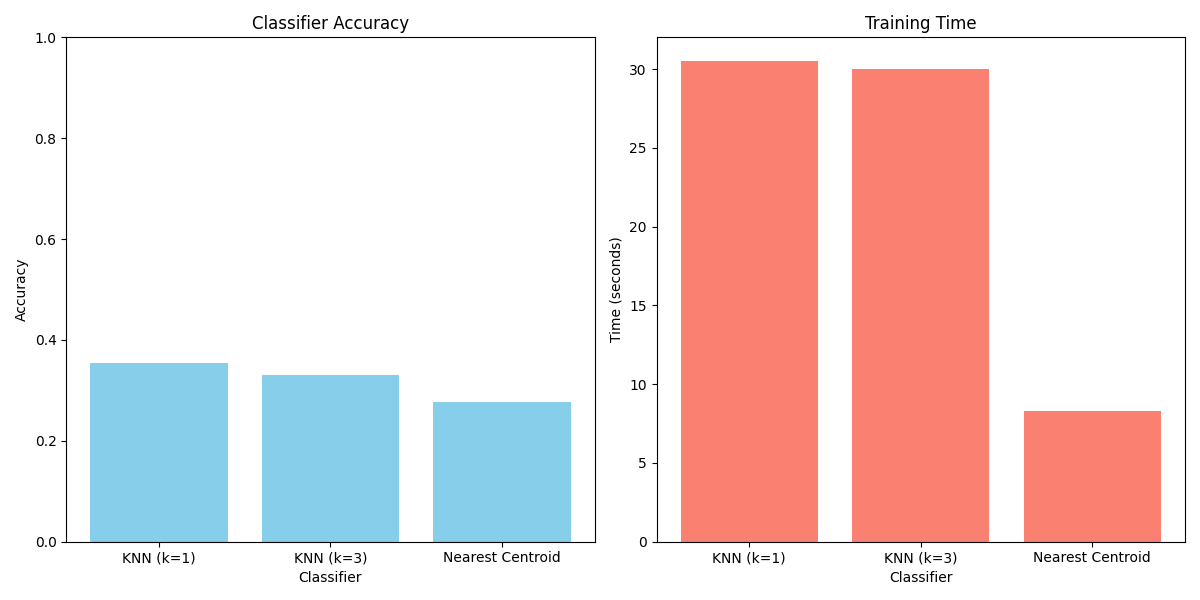
\includegraphics[width=0.5\textwidth]{media/knn_centroid.png}
    \caption{KNN Centroid Graph}
\end{figure}

Moving on to the MLP and CVM algorithms, it is important to note that
we are using:
\begin{itemize}
    \item A CPU as the training device
    \item Activation function: ReLU
    \item Loss function: Hinge loss
    \item Optimizer: Adam 
    \item Learning rate: 0.001
    \item Learning rate scheduler: ReduceLROnPlateau 
    \item Epochs: 30
    \item Training batch size: 128
    \item Testing batch size: 256
\end{itemize}

The graphs for both algorithms are as follows:
\begin{figure}[H]
    \centering
    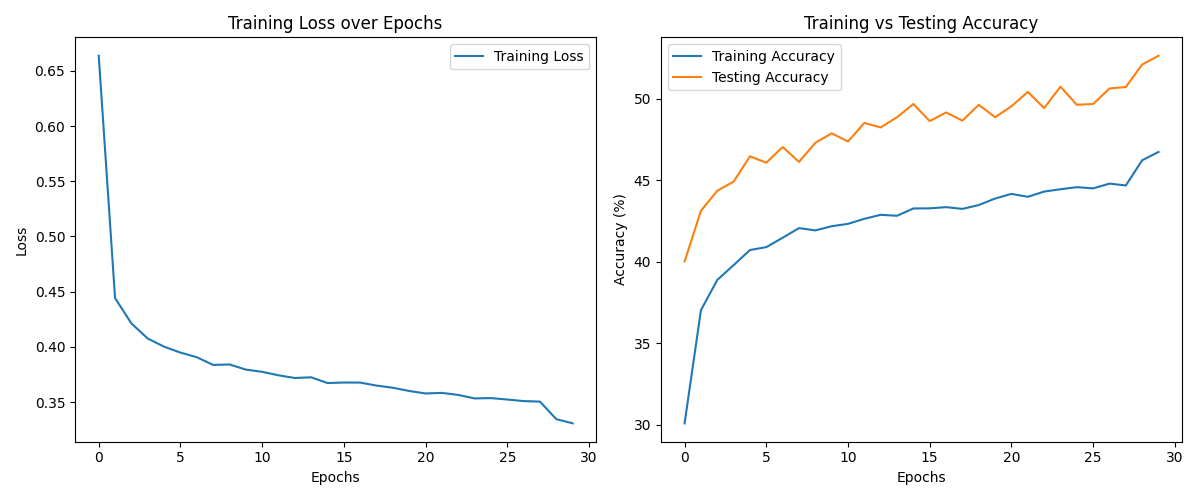
\includegraphics[width=0.5\textwidth]{media/mlp.png}
    \caption{MLP Graph}
\end{figure}

\begin{figure}[H]
    \centering
    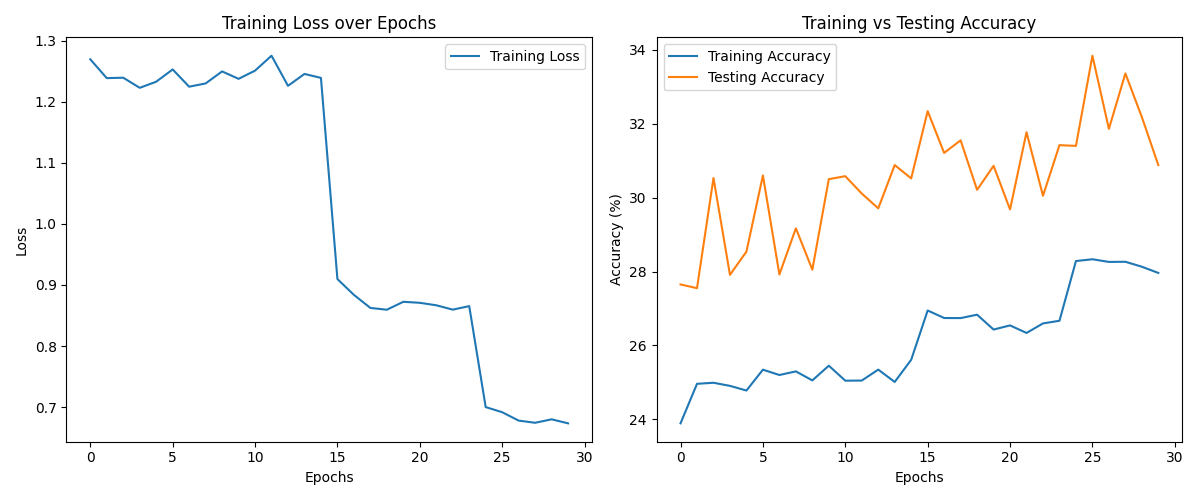
\includegraphics[width=0.5\textwidth]{media/svm.png}
    \caption{SVM Graph}
\end{figure}
Randomization filter like cropping and flipping improves the model's performance
but in return the training accuracy drops below the testing accuracy.\\

\smallskip

Lastly, the collective results showing the accuracies and times of
each algorithm, side by side, are as follows:
\begin{table}[H]
    \centering
    \begin{tabular}{|c|c|c|}
        \hline
        Algorithm & Accuracy & Time (seconds) \\
        \hline
        1-NN & 35.39 & 30.50 \\
        3-NN & 33.03 & 30.01 \\
        Nearest Centroid & 27.74 & 8.27 \\
        MLP & 52.63 & 1184.4 \\
        SVM & 33.84 & 321 \\
        \hline
    \end{tabular}
    \vspace{0.5cm}
    \caption{Comparison of Algorithms}
\end{table}

As an attempt to see if the algorithms have potential to rise in accuracy,
I increased the number of epochs:
\begin{figure}[H]
    \centering
    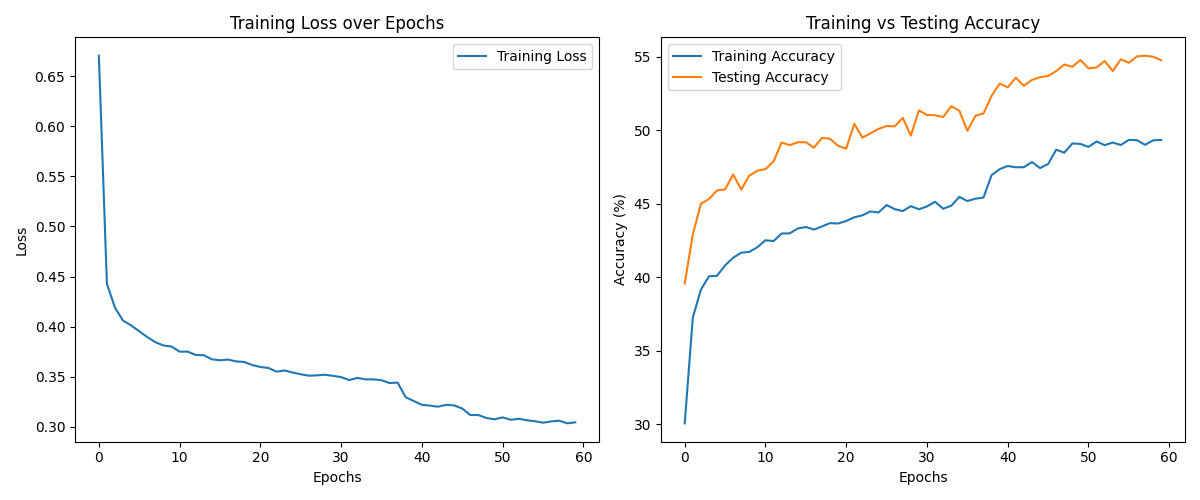
\includegraphics[width=0.5\textwidth]{media/mlp_max.png}
    \caption{MLP Graph - Extended Edition}
\end{figure}
Training completed in 43.65 minutes \\
Best accuracy: 55.08\% \\

\begin{figure}[H]
    \centering
    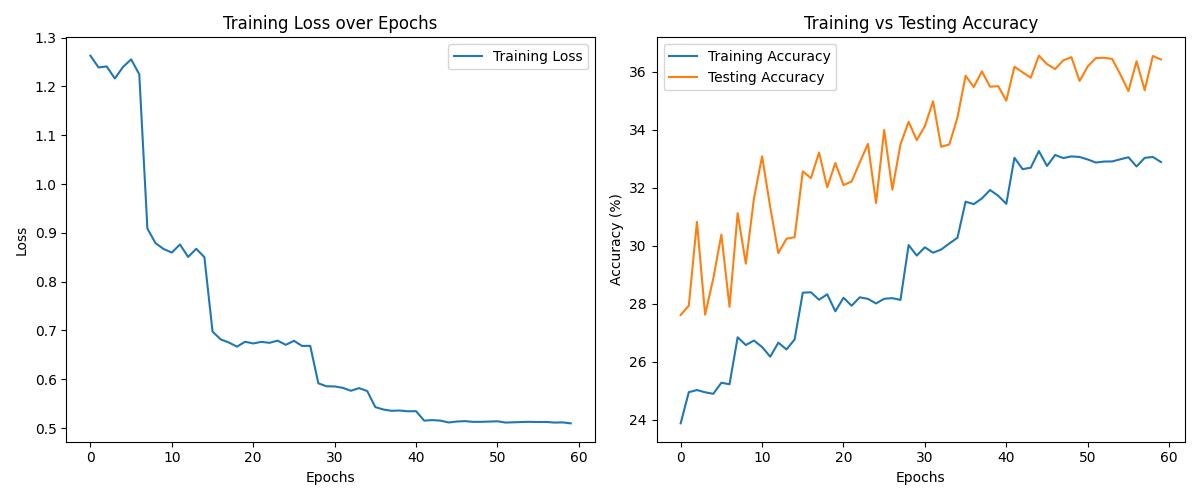
\includegraphics[width=0.5\textwidth]{media/svm_max.png}
    \caption{SVM Graph - Extended Edition}
\end{figure}
Training completed in 10.69 minutes \\
Best accuracy: 36.55\% \\

\smallskip

In the end the improvement was not significant.


\section{Modifications}
In order to improve the performance of the svm model I tried modifying the scheduler
and the optimizer. I noticed that using SDG with a StepLR scheduler I was able to 
surpass the accuracies of KNN and Nearest Centroid even though I was still behind MLP.
MLP has one hidden layer making it able to deal with more complex problems and thus 
it is expected to outperform the other algorithms. Here are the results of the SVM 
model with the modifications:
\begin{figure}[H]
    \centering
    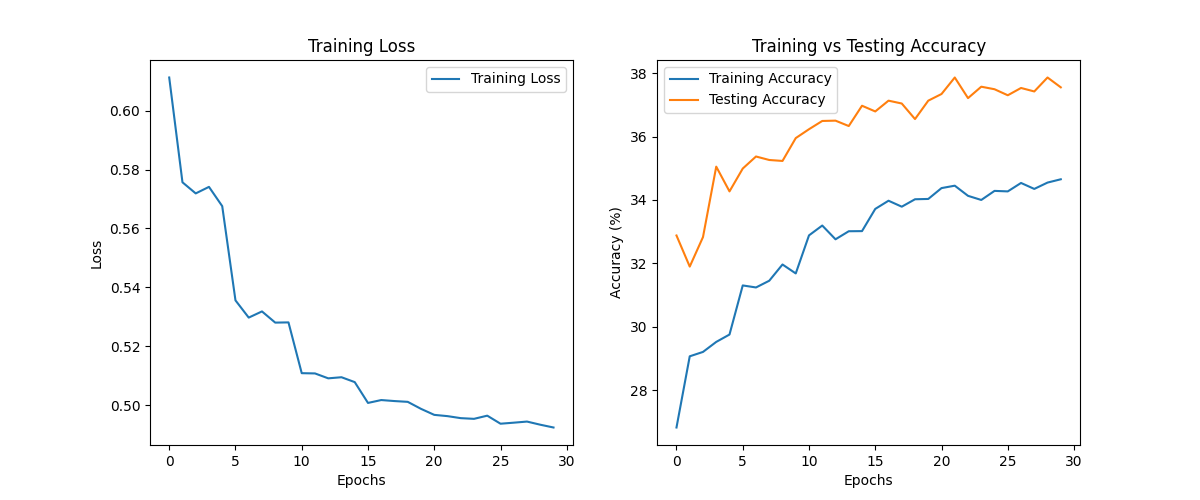
\includegraphics[width=0.5\textwidth]{media/svm_modified.png}
    \caption{SVM with SDG and StepLR scheduler}
\end{figure}
Training Completed in 5.35 minutes \\
Best Test Accuracy: 37.86\% \\

\smallskip

Let's break down why the performance improved, but first some general information
about the two SVM variations.
\begin{itemize}
    \item Adam optimizer with ReduceLROnPlateau scheduler
    \begin{itemize}
        \item Adam learning rate: 0.01
        \item ReduceLROnPlateau patience: 3
        \item ReduceLROnPlateau factor: 0.5
    \end{itemize}
    \item SGD optimizer with StepLR scheduler
    \begin{itemize}
        \item SGD learning rate: 0.01
        \item SGD weight decay: 0.0005
        \item SGD momentum: 0.9
        \item StepLR step size: 5
        \item StepLR gamma: 0.5
    \end{itemize}
\end{itemize}
Learning rates are kept the same for both optimizers to make the comparison fair.
They specify the step size at each iteration while moving toward a minimum of the 
loss function. The main difference between the two optimizers is that Adam is an 
adaptive learning rate optimization algorithm while SGD is a stochastic gradient 
descent algorithm. SGD has two additional parameters when compared to Adam:
\begin{itemize}
    \item Weight decay: Regularization term that penalizes large weights.
    \item Momentum: Accelerates the gradient descent by adding a fraction of the
    previous weight update to the current update. 
\end{itemize}

Reduce on Plateau is a scheduler that reduces the learning rate when a metric has 
stopped improving. In our case that metric is test\_loss. The scheduler has two 
important parameters:
\begin{itemize}
    \item Patience: Determines how many epochs to wait before reducing the learning 
    rate. 
    \item Factor: Determines how much to reduce the learning rate by.
\end{itemize}
On the other hand the StepLR scheduler reduces the learning rate by a factor every
fixed number of epochs. The scheduler has two important parameters:
\begin{itemize}
    \item Step size: Determines how many epochs to wait before reducing the learning 
    rate.
    \item Gamma: Determines how much to reduce the learning rate by.
\end{itemize}

Thus we can conclude based on our observations and the information above that the
SVM model is favored by a fixed scheduler and a stochastic gradient descent optimizer.
It has to be noted that reducing patience and factor on the Adam/ReduceLROnPlateau 
model did make the model learn faster and achieve slightly better accuracy in the end 
but it still lost to the StepLR scheduler. However, it isn't just the scheduler since 
Adam with the StepLR scheduler was once again 2\% behind the SDG/StepLR model. The 
fixed and steep learning rate reduction along with the momentum and weight decay
of the SGD marked a slight improvement in the performance of the SVM model, enough
to surpass KNN and Nearest Centroid.


\vfill
\end{document}


